\documentclass{article} % For LaTeX2e
\usepackage{nips14submit_e,times}
\usepackage{cite}
\usepackage{enumitem}
\usepackage{algorithm,algorithmicx}
\usepackage[noend]{algpseudocode}
\usepackage{url,graphicx,amsmath}
%\documentstyle[nips14submit_09,times,art10]{article} % For LaTeX 2.09
\usepackage[pagebackref=true,breaklinks=true,letterpaper=true,colorlinks,bookmarks=false]{hyperref}

\title{Project Report: User-Job Suitability Measurement}

\author{
XIN LIN \\
Department of Computer Science\\
University of Texas at Austin \\
Austin, TX 78705 \\
\texttt{jimmylin@utexas.edu} \\
%\And
%Coauthor \\
%Affiliation \\
%Address \\
%\texttt{email} \\
%\AND
%Coauthor \\
%Affiliation \\
%Address \\
%\texttt{email} \\
%\And
%Coauthor \\
%Affiliation \\
%Address \\
%\texttt{email} \\
%\And
%Coauthor \\
%Affiliation \\
%Address \\
%\texttt{email} \\
%(if needed)\\
}

% The \author macro works with any number of authors. There are two commands
% used to separate the names and addresses of multiple authors: \And and \AND.
%
% Using \And between authors leaves it to \LaTeX{} to determine where to break
% the lines. Using \AND forces a linebreak at that point. So, if \LaTeX{}
% puts 3 of 4 authors names on the first line, and the last on the second
% line, try using \AND instead of \And before the third author name.

\newcommand{\fix}{\marginpar{FIX}}
\newcommand{\new}{\marginpar{NEW}}

\nipsfinalcopy % Uncomment for camera-ready version

\begin{document}


\maketitle

\begin{abstract}

% Motivation
The essential part of job recommendation system is to evaluate suitability
between job seekers and available positions. However, currently popular job search
engines or job recommender systems online are weakly capable of providing
recommendation in intelligent ways. 
% overall formulation
This project formulates suitability
evaluation problem as an complicated system that prototyped from application
prediction and then transfer its power to suitability evaluation. 
% our contribution
For the the naive prototype, we apply recently emerged Inductive Matrix
Completion on task of predicting job seekers' application behavior. This new
approach significantly outshines other classic treatments. 
% dicussion section
Our discussion section at the end aims at giving several possible directions
of system extension in the future.
 
% For problem of application prediction:
%    0. inability of traditional binary classifier
%    1. demonstrate result of Inductive Matrix Completion 
%    2. compare it to other method - NN, one-class solver

% Discussion over how to augment this system

\end{abstract}

% TODO LIST:
% 2. apply IMC and do some fine-tune

% DONE LIST:
% 1. add description for each feature of user, job and application
% 2. apply inductive matrix completion (new) on job recommendation problem
% 3. compare IMC with old approaches, i.e. nearest neighbour and SVM.
% 4. discuss further enhancement of job recommender system.

% GENERALIZATION LIST:

\section{Introduction}
% Motivation
Job recommender system aims at helping people figure out a list of suitable
jobs and provide corresponding sugguestions if possible. However, exactly
modelling the suitability between users and jobs are challenging.

Due to the limitation of datasets, we experiment on application prediction for
initial setup and then find ways to reduce the problem to suitability
evaluation. 

\section{Problem Formulation}
If we assume that all job seekers are extremely knowledgeable (understand
clearly and completely the profile and requirement of every job) and rational
(never apply for the unsuitable jobs), we can directly makes use of the score
obtained in the application prediction. However, such assumption receives
little support from practical analysis, in the sense that people tend to apply
for the job positions with higher salaries and correspongly much more
capability seeking.

\subsection{Standarded Matrix Completion}
% explain binary suitability measurement
For startup, we first focus on binary suitability measurement problem. That
is, we only investigate the binary association, suitable (1) or not suitable
(0), for each pair of user and job. 
% Failure of traditional binary classifier
At first glance, this problem can be naively solved by traditional binary
classifiers, e.g. logistic regression and support vector machine, or one-class
learning solvers (or data description techniques).
Nevertheless, more carefull examination reveals obvious disadvantage of such
treatment. The main drawback of using traditional binary classifier is that.
% explain matrix completion formulation TODO

\subsubsection{Content-based Filtering}

\subsubsection{Collaborative Filtering}
The developing motivation of {\it Collaborative Filtering} is that the
profiles of items or users are not always available or poorly collect in
some settings but instead, the past histories of user-item association, also called {\it
    explicit feedback}, are easy to obtain. Collaborative filtering put its
focus directly on the target (user-job ), inferring missing ones from observed
one, rather than relationships between target
variables and features. Nearest neighbour method and latent factor model are
two major approaches for Collaborative Filtering.

% 2.1 nearest neighbour method TODO


% 2.2 latent factor model TODO
The latent factor model has an underlying assumption: the real exact rating matrix are
low-rank matrix. By modelling target rating variable as 
\begin{align}
    R_{ij} = u_i^T v_j 
\end{align}
we are able to use least square cost to guide the optimization procedure: 
\begin{align} \label{latent:opt}
    min \sum_{i,j} || r_{ij} - u_i^T v_j ||^2 
\end{align}
Note that $U \in R^{n\times k}$ and $V \in R^{m\times k}$ are respective matrices
restoring hidden-topic measurements for users and items(jobs). Intuitively,
$k$ denotes the number of latent topics, with its quantity reflecting shared
interest we want to measure over user and job entity. Also, regularized
squared error is typically used, in order to avoid overfitting of this model.
Hence, \ref{latent:opt} can be further extended to be 
\begin{align} \label{reglatent:opt}
    min \sum_{i,j} || r_{ij} - u_i^T v_j ||^2 + \lambda(||u_i||^2 + ||v_j||^2) 
\end{align}
One approach to get numerical solution is through {\it Stochastic Gradient
    Descent}, where each update take into account only one observed instance.
The update rules with $\gamma$ step size are presented as follows: 
\begin{align}
    v_j \leftarrow v_j + \gamma \big( (r_{ij}-u_i^T v_j)\cdot u_i + \lambda
    v_j \big) \\
    u_i \leftarrow u_i + \gamma \big( (r_{ij}-u_i^T v_j)\cdot v_j + \lambda
    u_i \big)
\end{align}
It can be easily figured out that equation \ref{reglatent:opt} is not convex.
But if we fix one variable ($U$ or $V$), the remained problem becomes convex
optimization and hence exact solution can be found. 
One alternative technique to solve \ref{reglatent:opt}, known as {\it Alternating
    Least Square}, takes advantage of this idea and turns out to be the one with
both computational convenience and convergence to decent local minima.

In netflix prize, the latent factor model, combined with temporal dynamics and
bias evaluation, winned as a single model with the greatest prediction power.
% 2.3 weakness 
Despite of that, collaborative filtering also has its limitation. It fails to
provide supervision of missing values when only rare amount of previous
association histories are provided, especially when the systems are on its
early stage.  This is commonly referred to as {\it cold startup} problem.

\subsection{One-Class Matrix Completion}

% add bias

\subsection{Inductive Matrix Completion}
% introduce this formulation and advantage of this framework
Comparing to collaborative filtering
, the conventional approach for matrix completion, advantages of incorporating
features are obvious in two aspects. One is lower sample complexity while
predicting missing values for known users and jobs.   The other is that precise
prediction can be produced for new/unkonw users and jobs. 

% brief math introduction
Formulate the problem as that of recovering a low-rank matrix $W_*$ using
observed entries $R_{ij} = x_i^T W_{*} y_j$ and the user/job feature vectors $x_i$, $y_j$. By
factoring $W = U V^T$ , we see that this scheme constitutes a bi-linear
prediction $(x^T U_{*})(V_{*} y)$ for a new user/job pair $(x, y)$.

% existing solver A (not scalable)
One practical solution is to use trace-norm constraint as a proxy for the rank
constraint and then solve the resulting non-smooth convex optimization
problem. Notwithstanding, the resulting convex optimization methods require
computation of full SVD for matrices with potentially large rank and hence do
not satisfy scalability to large problems.

% existing solver B (scalable but get stuck in local minima)
Parameterization over $W$ as $W = U V^T$ and then alternatingly optimize for
$U$ and $V$ is also a considerable approach in practice. To our best
knowledge, alternating minimization and its variants need to solve only least
squares problems and hence are scalable in practice but might get stuck in a
local minima.

% break through: dhillon's paper - inductive matrix completion
A recent paper \cite{jain2013provable} provides theoretical
supports for a variant of {\it alternating minimization} method to solve
{\it Inductive Matrix Completion} problem, in which other than a small number
of observations from the suitability matrix, the feature vectors for users and
jobs are also available.
According to \cite{jain2013provable}, under standard set of assumptions,
alternating minimization provably converges at a linear rate to the global
optimum of two low-rank estimation problems: a) RIP measurements based general
low-rank matrix sensing, and b) low-rank matrix completion. A more recent
paper \cite{natarajan2014inductive} in bioinformatics demonstrated successful
application of such inductive matrix completion
framework on gene-disease analytics.

% 3.2 propose kernel-based inductive matrix completion?
One possible enhancement for above inductive matrix completion is to
extend our consideration from the linear association between features and
latent factors to an version that accepts non-linear association.
By this intuition, we can name this approach as 
    {\it Kernel-based Inductive Matrix Completion}.
By taking into account non-linear relations between designed features and hidden
topics (shared latent factors), the space of latent factors can be largely
expanded and then it would be more likely to automatically detect latent
factors with higher quality. 
 
%\subsection{Scored Suitability Measurement (Multi-valued Version)}
%% this can also be used as a way of 
%A more elegant way to measure suitability between users and jobs is to
%directly predict scores based knowns. 

\subsection{Suitability Measurement with Prerequisites}
1. simulate course recommendaiton (by adita)

\section{Experiments: Application Prediction}
% introduce problem and evaluation criteria
Due to limitation of acquired data, our first experiment is oriented to
problem of application prediction. Specifically, given a set of featured users
and featured jobs, the designed system should predict whether one user will
apply for one particular job.

\subsection{Dataset}
% introduce experimented data set
The dataset utilized in this experimental project comes from a Job
Recommendation Challenge posted on
\href{http://www.kaggle.com/c/job-recommendation/data}{Kaggle.com}. The
provider of this dataset is
\href{http://www.careerbuilder.com/}{CareerBuilder.com}, one of the biggest
job recommendation service providers. This particular dataset, sized of several
Gigabytes, contains 389,708 featured users, 1,092,096
characterized jobs and 1,603,111 application records that are divided into
training and testing split.  In this section, we will at first provide the
fundamental introduction to these three basic elements: User, Job,
Application. And then explanation are illustrated about temporal separation (concept of
window) and designed distribution for user, job and application. 

% show details each record of user
As the most essential component of job recommendation system, users are
recorded by UserID, WindowID, Split, City, State, Country, ZipCode,
DegreeType, Major, GraduationDate, WorkHistoryCount,
TotalYearsExperience, CurrentlyEmployed, ManagedOthers, ManagedHowMany.
{\it UserID} refers to the nubmering index of that indicated user.  
{\it WindowsID} is about the timing period in which this particular
applicaiton about user happened. 
{\it City, State, Country, and ZipCode} are related to the living place of
that user. 
What follows are the achievements in school. 
{\it DegreeType} shows the highest degree that user has gained from school,
{\it Major} presents the field of his/her speciality and 
{\it GraduationDate} reveals when he/she gained the highest degree.
Working and management experience comes next.
{\it WorkHistoryCount} represents how many previous jobs one has had and
{\it TotalYearsExperience} represents how many years one has been involved in
occupation. 
{\it CurrentlyEmployed} and {\it ManagedOthers} are both binary values,
indicating whether one was currently on his/her job and whether he has been in
certain management position. 
{\it ManagedHowMany} implies his management power and capability, that is, the maximum number
of people he/she has managed before.

% show details each record of job
When it comes to information of every individual job, fields like JobID,
WindowID, Title, Description, Requirements, City, State, Country, Zip5,
StartDate, EndDate are provided.
{\it JobID} is the identifying number for each particular job. 
{\it WindowID} captures the same semantics as it is in a user record --
involved timing period of one job.
{\it Title} is the name of position sepcified by corresponding corporation, which
can be significantly important since it reflects relative position and power
in one company's hierarchy. 
Description and Requirements are both textual characterization
over each particular job. 
{\it Description} provides a
characteristic overview of one particular job. 
{\it Requirements} can be
viewed the basic expectation of hiring company towards the job applicants.
Similarly to the record of each individual user, every job also has location
information, such as {\it City, State, Country, ZipCode}. 
Besides, {\it StartDate} and {\it EndDate} shows the timing information of one job,
i.e. on which day it starts and ends. 

% show details each record of application
As to each instanced record of application, the dataset contains information
about the UserID, WindowID, Split, ApplicationDate, and JobID. 
{\it UserID} is indexing number of the user who applied for particular job,
indexed by {\it JobID}. 
{\it WindowID} implies the timing period of that application event, while
{\it ApplicationDate} presents the specific date of application event. 
And {\it Split} labelled in which division (training or testing set) that
piece of application was placed.

% explain the window ID
Next presented was the overall explanation about timing design of dataset. In
outline, all application instances span 13 weeks. All the job applications are
split into 7 groups, with each group representing a 13-day window. Each 13-day
window is split into two parts: The first 9 days are the training period, and
the last 4 days are the test period. The graphical representation
demonstrating such splits is illustrated below.
\begin{figure}[h]
    \begin{center}
        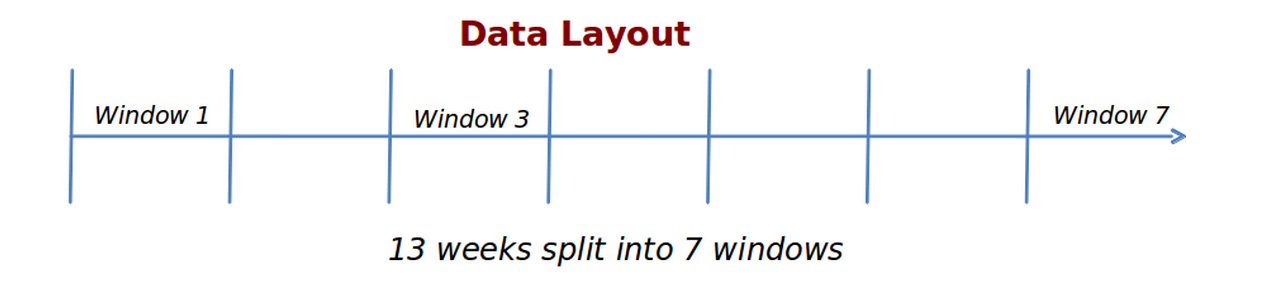
\includegraphics[width=4.3in,height=1.4in]{./fig/datalayout.png}
        \caption{Illustrating Diagram for Temporal Separation of the Dataset}
    \end{center}
\end{figure}

Note that each user and each job posting is randomly assigned to exactly one window.
Each job is assigned to a window with probability proportional to the time it
was live on the site in that window. Each user is assigned to a window with
probabilty proportional to the number of applications they made to jobs in
that window. As shown in the figure below, User1 only made submissions to jobs in
Window 1, and so was assigned to Window 1 with probability 100\%. User2,
however, made submissions to jobs in both Window 1 and Window 2, and so may
have been assigned to either Window1 or Window2.

\begin{figure}[h]
    \begin{center}
        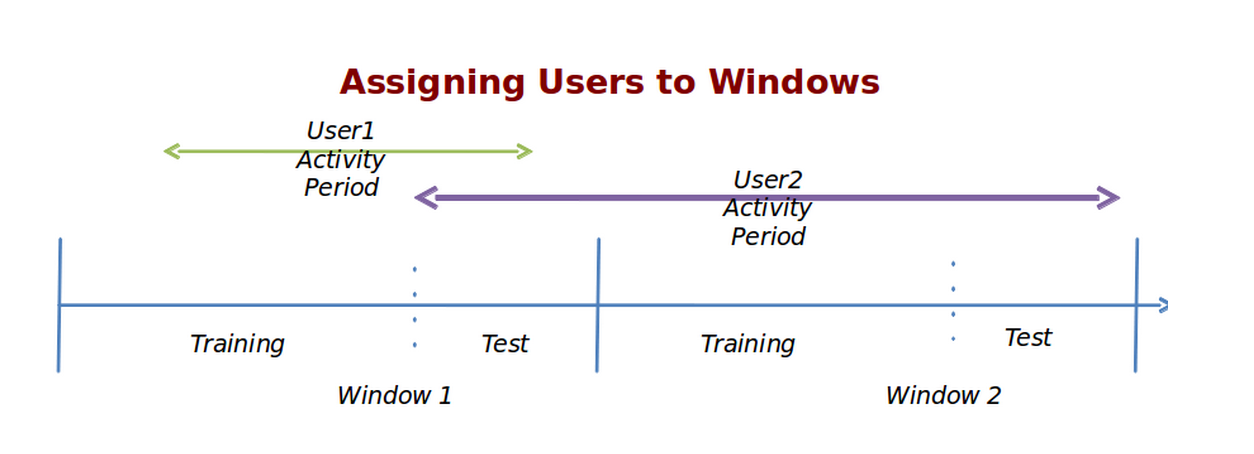
\includegraphics[width=4.3in,height=1.8in]{./fig/assignusertowindows.png}
        \caption{Explanation for user distribution}
    \end{center}
\end{figure}

In each window, all the job applications that users in that window made to
jobs in that window during the 9-day training period. 
And with each window, users have been split into two groups, {\it Test group}
and {\it Train group}. The Test users are those who made 5 or more
applications in the 4-day test period, and the Train users are those who did
not.

For each window, the task of prediction is which jobs in that window the Test
users applied for during the window's test period. Note that users may have
applied to jobs from other windows as well, but the only thing needed to be
predicted is which jobs they applied to in their own windows.

% TODO:some key observation from dataset

\subsection{Preprocessing} % ways to preprocessing
Preprocessing, as the earliest step for any machine learning
experimentation, is extremely important in that it, as a role of filter, 
process the raw data and then generates what is later employed by human-design
AI system. From this perspective, any inconsistent or invalid processing would
cause devastating effects for the entire system.

% 0. instance subsetting
{\bf Instance Subsetting}.
Since there are huge quantities of users and jobs, our experiment only
exploits the first part of dataset (WindowsID = 1) for computational
convenience. Another benefit for such instance subsetting is to temporarily
put aside the temporal dynamics, that is, disregard the impact of timing
variable for now. And the investigation over how to accommodate the designed system
to the entire dataset can be deferred to later study.

% 1. binary encoding of discrete value
{\bf Binary Encoding Scheme}.
For all nominal attributes, we represent every of them as a collection of binary
variables. For example, DegreeType, indicating the highest
degree obtained by one user, has five possible values: None, High
School, Bachelor, Master, PhD. We have five binary variables indicating if one
user has highest degree on None, High School, Bachelor, Master, PhD
respectively. Other examples of such nominal attributes in this application
prediction problem are Zip5, City, State and Country. 
One advantage of such processing lies in multi-valued features, like Major.
Some people may be double-major or even three-major. 
In these cases, no conflict would occur if we apply take binary encoding
scheme. However, the binary encoding scheme will significantly augment the scale of
learning task since some nominal attributes have huge domain dimensionality.
Hence, it is unavoidable to leave out redundant attributes. 

% 2. feature subsetting (user, job, application)
{\bf Attributes Subsetting}.
To simplify initial setup of this machine learning experimentation, we
manually left out some three categories of attributes. First category is
semantically meaningless information. On top of that, those attributes that may contribute to
application prediction (slightly higher accuracy) but overwhelmingly enlarge
the scale of learning (significantly lower speed) are also eliminated for now.
Zip5 is the most illustrative example for this type of attribute.
Another set of attributes are disregarded because we are incapable of
modelling these relevant factors. For example, temporal dynamics (i.e. {\it
    StartDate and EndDate} of job) are not planned to be captured in our
current design. 

% 3. processing textual data (description, requirements)
%% (present procedure)
{\bf Efficient Representation of Textual Data}.
The ways to process textual data are important because we hope to narrow the
scale of numerical representation for these texts.  The sequential procedures
of processing raw text data are specified as follows:
\begin{enumerate}[label=(\roman*)]
  \item{Convert all terms into lowercase.}
  \item{Eliminate stop words.}
  \item{Annihilate all meaningless terms with particular forms, i.e.
          timestamps, datestamps, IP addresses, phone numbers and webpage link}
  \item{Remove all punctuations.}
  \item{Check validity of words.}
  \item{Acquires linguistic stemmes for each tokens. This step also removes
          plurals and tenses.}
\end{enumerate}
%% (present statistics of product)
As a consequence of applying above transformations, {\bf 12841}
keywords (distinct vocabularies) are obtained. 

% 4. data format of preprocessing product 
{\bf Preprocessing Products}.
Through preprocessing, we generate three data files for later machine learning
algorithm: {\it win1\_Users.sparse, win1\_Jobs.sparse and win1\_Apps.sparse}.
Within {\it win1\_Users.sparse}, there are $77060$ users with $1416$ features per
user. {\it win1\_Jobs.sparse} maintained records of $285515$ jobs, each of
which has $12841$ features for now. {\it win1\_Apps.sparse} contains a sparse
matrix with dimensionality $77060\times285515$.

{\bf Storage Format} Note that all numerics generated by preprocessing procedure are restored as libSVM
format in that the generated features for user and job have huge extent of sparsity. 
Specifically, for every job or user contained in win1\_Users.sparse,
win1\_Jobs.sparse, the representation of each object is as follows:
\begin{center}
    feature\_index:feature\_value \ feature\_index:feature\_value .... 
\end{center}
On the other hand, the representation for each application instance is slightly different,
but still in standarded LibSVM format. 
\begin{center}
    apply\_or\_not 0:user\_index 1:job\_index
\end{center}

\subsection{Failure of Traditional Binary Classifiers} % 0.5 page
As we can observe from the dataset, all "not apply" behaviors of users are
missing and hence the dataset cannot supervise the learning of "not apply"
behavior of users. It is easy to conclude that all traditional binary
classifiers, including logistic regression and classic support vector machine,
fail to work in this setting.

And more intuitive failure occurs to nearest neighours model. Typically to
predict application of one user and one job, we can look up the k most similar
users or k most similar jobs in terms of their features. Nevertheless, under
this one-class setting, no neibours of negative class can provide a negative
support on the majority voting.

\subsection{Standarded One-Class Matrix Completion}
Due to the observation that only behaviors of "apply" are recorded in the
dataset, one-class problem, where only instances of positive classes are
supervised in the training, naturally come to our mind.

\subsubsection{One-class Matrix Completion} % 0.5 page

\subsubsection{One-class Matrix Completion with Bias} % 0.5 page

\subsubsection{Weakness}

\subsection{Inductive Matrix Completion} % 1-2 pages

As previously mentioned, one should formulate it as {\it inductive matrix
    completion} when side information of users and items (in this case, jobs)
are available. 
Even through simple alternating minimization method, one should be able to
recover back the exact underlying low-rank matrix and predict inductively on
new users and jobs if provided conditions are satisfied by the set of
measurements \cite{jain2013provable}. 
And intuitively, it is not exaggerated to claim that such formulation and
corresponding solver (AltMin) take advantage of both classic approaches -- content-based
filtering and collaborative filtering in recommendation problem: 
    less sample complexity and inductivity on new users/jobs. 

\subsubsection{Algorithmic Description} 
% algorithm presentation
\newcommand{\xii}{\boldsymbol{x}_i}
\newcommand{\yj}{\boldsymbol{y}_j}
The algorithmic procedures are shown in Algorithm \ref{alg:AltMin}.
\begin{algorithm}
    \caption{Alternating Minimization for Least-Square Inductive Matrix
        Completion}
    \label{alg:AltMin}
    \begin{algorithmic}[1]

\State \textbf{INPUT}: \\ \ \ a) sparse matrices $X$ and $Y$ denote features of users
and jobs. \\ \ \ b) matrix $A$ denotes partial observation of application
association with observed index set $\Omega$
\State \

\State Initialize $U_{(0)}$ and $V_{0}$ by uniform randomization
\State \textbf{Do}  
\State \  \
    $V_{(k+1)}$ = argmin $\alpha \sum_{(i,j) \in \Omega} 
    (\xii^T U_{(k)} V_{(k)}^T \yj - 1)^2 
    + (1-\alpha) \sum_{(i,j) \not \in \Omega} (\xii^T U_{(k)} V_{(k)}^T \yj - 0)^2$

\State \  \
$U_{(k+1)}$ = argmin $\alpha \sum_{(i,j) \in \Omega}(\xii^T
    U_{(k)} V_{(k+1)}^T \yj - 1)^2 +
    (1-\alpha) \sum_{(i,j) \not \in \Omega}(\xii^T U_{(k)} V_{(k+1)}^T \yj - 0)^2$
\State \textbf{Until} Convergence. 
\State Predict values for missing entries: $\forall (i,j) \not \in \Omega$, 
$R_{ij} = \xii^T U_{*} V_{*}^T \yj$

\State \

\State \textbf{OUTPUT: } \\ 
\ \ a) Model Parameter $ U_{*}$ and $V_{*}$ 
\end{algorithmic}
\end{algorithm}

\textbf{Bias}. Bias parameter $\alpha \in (0, 1)$ is the weight to balance
optimization objective between observed and missing labels. Note that with
unbiased version of inductive one-class matrix completion, this parameter
should be set to $1$, that is $\alpha = 1$.

\textbf{Initialization}. Randomizing all components of $U_{(0)}$ and
$V_{(0)}$ to uniform distribution over $(0, 1)$ works well in our
experimentation. 

\textbf{Optimization}.
During each stage of alternating minimization, standarded conjugate gradient method is
employed to solve least square problem. 

\subsubsection{Inductive One-Class Matrix Completion} % 0.5 pages

\subsubsection{Inductive One-Class Matrix Completion with Bias} 

\subsubsection{Results}
% one graph to demonstrate the result (error w.r.t lambda)


\subsection{Conclusions}
% one concluding paragraph

% \subsection{ (optional) kernelized inductive matrix completion}

\section{Experiments: Suitability Evaluation}
We now start to divert our focus on investigating Application Potential to
Suitability Evaluation.

\section{Discussions}

%\subsubsection*{References}
\bibliography{main}{}
\bibliographystyle{plain}


\end{document}
